\documentclass[aspectratio=169]{beamer}

%% ── Theme & colours ─────────────────────────────────────────────────────────
\usetheme{Madrid}
\usecolortheme{seahorse}
\setbeamertemplate{navigation symbols}{}
\setbeamertemplate{footline}[frame number]

%% ── Packages ────────────────────────────────────────────────────────────────
\usepackage{amsmath,amssymb}
\usepackage{bm}
\usepackage{booktabs}
\usepackage{graphicx}
\usepackage{tikz}
\usepackage{xcolor}
\usepackage{hyperref}

\graphicspath{{../../results/}}

%% ── Custom commands ─────────────────────────────────────────────────────────
\newcommand{\E}{\mathbb{E}}
\newcommand{\R}{\mathbb{R}}
\newcommand{\1}{\mathbf{1}}
\newcommand{\dB}{\delta_{\mathrm{bid}}}
\newcommand{\dA}{\delta_{\mathrm{ask}}}

%% ── Title information ───────────────────────────────────────────────────────
\title[RL for Market Making]{\textbf{Reinforcement Learning for Market Making}}
\subtitle{Dynamic Programming vs.\ Deep Q-Networks}
\author{Sam \and Siddhant \and Sondre}
\date{\today}
\institute{RL Book Course Project}

% ═════════════════════════════════════════════════════════════════════════════
\begin{document}

\begin{frame}
  \titlepage
\end{frame}

\begin{frame}{Outline}
  \tableofcontents
\end{frame}

% ─────────────────────────────────────────────────────────────────────────────
\section{Overview}
% ─────────────────────────────────────────────────────────────────────────────

\begin{frame}{What is Market Making?}
  \begin{columns}[T]
    \column{0.55\textwidth}
      \textbf{Market maker's role:}
      \begin{itemize}
        \item Continuously posts \textbf{bid} (buy) and \textbf{ask} (sell) quotes
        \item Earns the \emph{bid--ask spread} on each filled trade
        \item Bears \textbf{inventory risk}: holding assets in a volatile market
      \end{itemize}
      \vspace{1em}
      \textbf{Core tension:}
      \begin{itemize}
        \item \emph{Tight spreads} $\Rightarrow$ more order flow but more risk
        \item \emph{Wide spreads} $\Rightarrow$ less risk but fewer trades
        \item Optimal quoting depends on \textbf{inventory}, \textbf{price}, \textbf{volatility}
      \end{itemize}
    \column{0.42\textwidth}
      \centering
      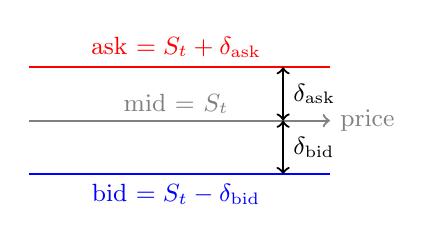
\begin{tikzpicture}[scale=0.85, every node/.style={font=\small}]
        % Mid price
        \draw[thick, ->, gray] (0,0) -- (4.5,0) node[right]{price};
        \node[gray] at (2.2, 0.25) {mid = $S_t$};
        % Bid
        \draw[blue, thick] (0, -0.8) -- (4.5, -0.8);
        \node[blue] at (2.2, -1.1) {bid $= S_t - \dB$};
        % Ask
        \draw[red, thick] (0, 0.8) -- (4.5, 0.8);
        \node[red] at (2.2, 1.1) {ask $= S_t + \dA$};
        % Arrows
        \draw[<->, thick] (3.8, 0) -- (3.8, 0.8) node[midway, right]{$\dA$};
        \draw[<->, thick] (3.8, -0.8) -- (3.8, 0) node[midway, right]{$\dB$};
      \end{tikzpicture}
      \vspace{0.5em}

      \textit{Profit per fill $\approx \delta_{\mathrm{bid}}$ or $\delta_{\mathrm{ask}}$}
  \end{columns}
\end{frame}

\begin{frame}{Our Approach: RL + DP Comparison}
  \begin{block}{Goal}
    Train a market-making agent to dynamically set bid/ask spreads using\\
    \textbf{Reinforcement Learning (DQN)} and compare with \textbf{Dynamic Programming (Value Iteration)}.
  \end{block}

  \vspace{0.5em}
  \textbf{Three progressively richer experiments:}
  \begin{enumerate}
    \item \textbf{Exp 1} — Inventory-only state, constant volatility
    \item \textbf{Exp 2} — (Inventory, Price) state, constant volatility
    \item \textbf{Exp 3} — (Inventory, Price, Volatility) state, stochastic volatility
  \end{enumerate}

  \vspace{0.5em}
  \begin{alertblock}{Key question}
    When does DP \emph{fail} (curse of dimensionality), and when does RL succeed?
  \end{alertblock}
\end{frame}

% ─────────────────────────────────────────────────────────────────────────────
\section{Method}
% ─────────────────────────────────────────────────────────────────────────────

\begin{frame}{MDP Formulation — Common Setup}
  \textbf{Actions:} asymmetric spread pairs
  \[
    a_t = (\dB,\, \dA) \in \{0.5,\; 1.0,\; 1.5\}^2 \quad (9 \text{ actions})
  \]

  \textbf{Fill probabilities} (Poisson order arrivals):
  \[
    \lambda(\delta) = A\,e^{-k\delta}, \qquad
    P(\text{fill on side } s) = 1 - e^{-\lambda(\delta_s)}
  \]

  \textbf{Price dynamics} (with adverse selection):
  \[
    \Delta S_t = \underbrace{\alpha_{\mathrm{adv}}\bigl(\1_{\mathrm{ask\,fill}} - \1_{\mathrm{bid\,fill}}\bigr)}_{\text{adverse selection}} + \;\sigma_t\,\varepsilon_t, \quad \varepsilon_t \sim \mathcal{N}(0,1)
  \]

  \textbf{Reward:}
  \[
    r_t = \underbrace{\dB\,\1_{\mathrm{bid}} + \dA\,\1_{\mathrm{ask}}}_{\text{spread capture}}
          + \underbrace{I_t \cdot \Delta p_{\mathrm{det}}}_{\text{inventory P\&L}}
          - \underbrace{\alpha\, I_t^2}_{\text{inv.\ penalty}}
  \]

  \textbf{Discount factor:} $\gamma = 0.99$, \textbf{Inventory bound:} $I_t \in \{-5,\ldots,5\}$
\end{frame}

\begin{frame}{Experiment 1 — Inventory-Only State}
  \begin{columns}[T]
    \column{0.48\textwidth}
      \textbf{State space:}
      \[
        s_t = I_t \in \{-I_{\max},\ldots,I_{\max}\} \quad (11 \text{ states})
      \]

      \textbf{Volatility:} constant $\sigma$

      \vspace{0.5em}
      \textbf{Bellman equation (DP):}
      \[
        V(I) = \max_{a}\;\E\bigl[r(I,a) + \gamma\,V(I')\bigr]
      \]
      Solved via \textbf{value iteration} ($11 \times 9$ table).

      \vspace{0.5em}
      \textbf{RL:} DQN with one-hot inventory encoding\\
      \quad $\to$ state dim = 11, output dim = 9

    \column{0.48\textwidth}
      \textbf{Why this works for DP:}
      \begin{itemize}
        \item Small, discrete state space
        \item Known transition dynamics
        \item Exact solution in seconds
      \end{itemize}

      \vspace{0.5em}
      \textbf{Intuition:}
      \begin{itemize}
        \item High $I$ $\Rightarrow$ want to sell $\Rightarrow$ tight ask, wide bid
        \item Low $I$ $\Rightarrow$ want to buy $\Rightarrow$ tight bid, wide ask
        \item Zero $I$ $\Rightarrow$ symmetric spreads
      \end{itemize}
  \end{columns}
\end{frame}

\begin{frame}{Experiment 2 — Adding Price to State}
  \begin{columns}[T]
    \column{0.48\textwidth}
      \textbf{State space:}
      \[
        s_t = (I_t,\; S_t) \quad \text{with } S_t \in [-5, 5]
      \]
      Price discretised into $21$ bins $\Rightarrow$ $11 \times 21 = \mathbf{231}$ states

      \vspace{0.5em}
      \textbf{DP:} 2-D value iteration
      \[
        V(I, S) = \max_{a}\;\E\bigl[r + \gamma\,V(I', S')\bigr]
      \]

      \textbf{RL:} DQN with one-hot $(I, S)$ encoding\\
      \quad $\to$ state dim = $11 + 21 = 32$

    \column{0.48\textwidth}
      \textbf{Additional insight from price:}
      \begin{itemize}
        \item Lower price $\Rightarrow$ smaller absolute spreads\\
          (price moves proportional to price level)
        \item DP still tractable: $231 \times 9$ table
        \item Policy is now a \emph{2-D heatmap} over $(I, S)$
      \end{itemize}

      \vspace{0.5em}
      \begin{alertblock}{DP vs.\ RL distinction}
        DP \emph{discretises} price to make it tractable.
        RL can, in principle, handle continuous price natively.
      \end{alertblock}
  \end{columns}
\end{frame}

\begin{frame}{Experiment 3 — Adding Stochastic Volatility}
  \begin{columns}[T]
    \column{0.48\textwidth}
      \textbf{State space:}
      \[
        s_t = (I_t,\; S_t,\; \sigma_t)
      \]
      $\sigma_t$ follows an \textbf{Ornstein--Uhlenbeck} process:
      \[
        \Delta\sigma_t = \kappa(\theta - \sigma_t) + \xi\,\varepsilon_t^v
      \]
      with $\kappa = 0.15$, $\theta = 0.2$, $\xi = 0.2$.

      \vspace{0.5em}
      Volatility discretised into $9$ bins $\in [0.3, 2.0]$\\
      $\Rightarrow$ $11 \times 15 \times 9 = \mathbf{1{,}485}$ states

    \column{0.48\textwidth}
      \textbf{DP:} 3-D value iteration (still tractable, but slow)

      \textbf{RL:} DQN with one-hot encoding\\
      \quad $\to$ state dim = $11 + 15 + 9 = 35$

      \vspace{0.5em}
      \textbf{New dynamic:}
      \begin{itemize}
        \item High $\sigma$ $\Rightarrow$ more conservative (wider spreads)
        \item Inventory risk amplified by volatility
        \item Policy now a \emph{3-D object}: $V(I, S, \sigma)$
      \end{itemize}

      \vspace{0.5em}
      \textbf{Curse of dimensionality:}
      Adding one more continuous feature (e.g.\ regime, $\lambda$) would make DP intractable --- RL becomes necessary.
  \end{columns}
\end{frame}

\begin{frame}{DP vs.\ RL: Algorithms}
  \begin{columns}[T]
    \column{0.48\textwidth}
      \textbf{Dynamic Programming} (Value Iteration)
      \begin{itemize}
        \item Requires \emph{known} transition model $P(s'|s,a)$
        \item Sweeps over all states until convergence:
          \[
            V_{k+1}(s) \leftarrow \max_a\sum_{s'}P(s'|s,a)\bigl[r + \gamma V_k(s')\bigr]
          \]
        \item Exact, guaranteed convergence
        \item Scales as $\mathcal{O}(|\mathcal{S}|^2|\mathcal{A}|)$ per sweep
        \item \textbf{Fails} when $|\mathcal{S}|$ is large or continuous
      \end{itemize}

    \column{0.48\textwidth}
      \textbf{Reinforcement Learning} (DQN)
      \begin{itemize}
        \item \emph{Model-free}: learns from environment interactions
        \item Approximates $Q(s,a) \approx Q_\theta(s,a)$ with a neural network
        \item TD update (experience replay):
          \[
            \mathcal{L} = \bigl(r + \gamma \max_{a'} Q_{\bar\theta}(s',a') - Q_\theta(s,a)\bigr)^2
          \]
        \item Works with large / continuous state spaces
        \item Sample-inefficient, sensitive to hyperparameters
      \end{itemize}
  \end{columns}

  \vspace{0.5em}
  \begin{block}{Project emphasis}
    Experiments 1--3 demonstrate when DP is sufficient and when RL is the better tool.
  \end{block}
\end{frame}

\begin{frame}{Environment Details}
  \begin{columns}[T]
    \column{0.48\textwidth}
      \textbf{Order flow model:}
      \begin{itemize}
        \item Arrival rate: $\lambda(\delta) = 0.5\,e^{-1.5\,\delta}$
        \item Independent Poisson processes per side
        \item Inventory capped at $|I| \leq 5$
      \end{itemize}

      \vspace{0.5em}
      \textbf{Adverse selection:}
      \begin{itemize}
        \item Ask fill $\Rightarrow$ price tends to rise by $\alpha_{\mathrm{adv}} = 0.2$
        \item Bid fill $\Rightarrow$ price tends to fall by $0.2$
        \item Simulates informed traders
      \end{itemize}

    \column{0.48\textwidth}
      \textbf{Reward:}
      \[
        r_t = \dB\,\1_{\mathrm{bid}} + \dA\,\1_{\mathrm{ask}} + I_t\,\Delta S_t - \alpha I_t^2
      \]
      Full mark-to-market inventory P\&L $I_t \Delta S_t$ including the noisy $\sigma_t \varepsilon_t$ component.

      \vspace{0.5em}
      \textbf{Challenge:} $I_t \cdot \sigma_t \varepsilon_t$ has SNR $\approx 0.5$,\\
      drowning the spread signal --- making it hard for RL to distinguish good from bad actions.

      \vspace{0.5em}
      \textbf{Episode:} $T = 200$ steps, $\gamma = 0.99$
  \end{columns}
\end{frame}

% ─────────────────────────────────────────────────────────────────────────────
\section{Results}
% ─────────────────────────────────────────────────────────────────────────────

\begin{frame}{Key Findings}
  \begin{enumerate}
    \item \textbf{Low signal-to-noise ratio is the core challenge}
    \begin{itemize}
      \item Price volatility $\sigma \varepsilon$ swamps the spread signal
      \item Suboptimal policies achieve nearly the same PnL as optimal --- RL struggles to differentiate Q-values
    \end{itemize}

    \vspace{0.4em}
    \item \textbf{Optimal policy is inventory-driven}
    \begin{itemize}
      \item High inventory $\Rightarrow$ tight ask (incentivise selling), wide bid
      \item Low inventory $\Rightarrow$ tight bid (incentivise buying), wide ask
    \end{itemize}

    \vspace{0.4em}
    \item \textbf{Price level affects spread magnitude}
    \begin{itemize}
      \item Lower price $\Rightarrow$ smaller spreads (price moves scale with price)
    \end{itemize}

    \vspace{0.4em}
    \item \textbf{Volatility induces conservatism}
    \begin{itemize}
      \item High $\sigma$ $\Rightarrow$ wider spreads to compensate for inventory risk
    \end{itemize}
  \end{enumerate}
\end{frame}

\begin{frame}{Experiment 1 Results: Inventory-Only State}
  \begin{center}
    
\includegraphics[width=0.82\textwidth]{exp1_comparison.png}
  \end{center}
\end{frame}

\begin{frame}{Experiment 2 Results: (Inventory, Price) State}
  \begin{center}
    
\includegraphics[width=0.82\textwidth]{exp2_comparison.png}
  \end{center}
\end{frame}

\begin{frame}{Experiment 2 Policy Heatmaps}
  \begin{center}
    
\includegraphics[width=0.82\textwidth]{exp2_policy_heatmap.png}
  \end{center}
\end{frame}

\begin{frame}{Experiment 3 Results: (Inventory, Price, Vol) State}
  \begin{center}
    
\includegraphics[width=0.82\textwidth]{phase3_comparison.png}
  \end{center}
\end{frame}

\begin{frame}{Experiment 3 Policy Heatmaps}
  \begin{center}
    
\includegraphics[width=0.82\textwidth]{phase3_policy_heatmap.png}
  \end{center}
\end{frame}

% ─────────────────────────────────────────────────────────────────────────────
\section{Conclusion}
% ─────────────────────────────────────────────────────────────────────────────

\begin{frame}{Summary of Experiments}
  \begin{table}
    \centering
    \small
    \begin{tabular}{lcccc}
      \toprule
      & \textbf{State} & \textbf{DP tractable?} & \textbf{RL needed?} & \textbf{States} \\
      \midrule
      Exp 1 & $I$ only            & \checkmark (trivial)   & Optional  & 11 \\
      Exp 2 & $(I, S)$            & \checkmark (manageable)& Optional  & 231 \\
      Exp 3 & $(I, S, \sigma)$    & \checkmark (slow)      & Preferred & 1{,}485 \\
      Full model & + regime, $\lambda$, \ldots & $\times$ (intractable) & \textbf{Required} & $\infty$ \\
      \bottomrule
    \end{tabular}
  \end{table}

  \vspace{0.7em}
  \begin{itemize}
    \item \textbf{Exp 1:} DP and RL both recover the inventory-hedging policy; RL converges after $\sim$3M steps.
    \item \textbf{Exp 2:} Price dimension adds a new policy gradient --- lower prices $\Rightarrow$ tighter spreads. DP solves the 2-D table exactly; RL matches qualitatively.
    \item \textbf{Exp 3:} Stochastic volatility is key: the OU process drives the agent to widen spreads at high $\sigma$. DP requires careful discretisation and becomes computationally expensive. RL scales more gracefully.
  \end{itemize}
\end{frame}

\begin{frame}{Takeaways}
  \begin{block}{DP is exact but limited}
    Requires full model knowledge and a small, discrete state space. As state dimensions grow, the curse of dimensionality makes DP impractical.
  \end{block}

  \vspace{0.5em}
  \begin{block}{RL is flexible but hard to train}
    Model-free and scales to large/continuous states, but suffers from low SNR in noisy environments --- the spread signal is easily buried by price volatility.
  \end{block}

  \vspace{0.5em}
  \begin{block}{Market making is a canonical RL challenge}
    The optimal policy has clear intuitive structure (inventory mean-reversion, volatility-adaptive spreads), but the reward signal is weak relative to environmental noise --- motivating careful reward shaping and training design.
  \end{block}
\end{frame}

\begin{frame}[plain]
  \begin{center}
    \vspace{2cm}
    {\Huge \textbf{Questions?}}\\[2em]
    {\large Sam \quad Siddhant \quad Sondre}
  \end{center}
\end{frame}

\end{document}
